\documentclass[a4paper]{article}
\usepackage{student}
\usepackage{hyperref}
\usepackage{graphicx}
\usepackage{algorithm}
\usepackage{algorithmic}
\usepackage{breqn}
\usepackage{subcaption}
\usepackage{multirow}
\usepackage{psfrag}
\usepackage{url}
\usepackage{hyperref}
%\usepackage[colorlinks]{hyperref}
\usepackage{cleveref}
\usepackage{booktabs}
\usepackage{rotating}
\usepackage{colortbl}
\usepackage{paralist}
%\usepackage{geometry}
\usepackage{epstopdf}
\usepackage{nag}
\usepackage{microtype}
\usepackage{siunitx}
\usepackage{nicefrac}
% for random text
\usepackage{lipsum}
\usepackage[english]{babel}
\usepackage[pangram]{blindtext}
% for tikz figures
\usepackage{listings}
\usepackage{tikz}
\usetikzlibrary{fit,positioning,arrows.meta,shapes,arrows}
% Metadata
\date{\today}
\setmodule{SIT742: Modern Data Science}
\setterm{Trimester 2, 2023}

%-------------------------------%
% Other details
% TODO: Fill these
%-------------------------------%
\title{Assignment 1}
\setmembername{SIT742}  % Fill group member names
%\setmemberuid{u1234567, u7654321}  % Fill group member uids (same order)

%-------------------------------%
% Add / Delete commands and packages
% TODO: Add / Delete here as you need
%-------------------------------%
\usepackage{amsmath,amssymb,bm}

\newcommand{\KL}{\mathrm{KL}}
\newcommand{\R}{\mathbb{R}}
\newcommand{\E}{\mathbb{E}}
\newcommand{\T}{\top}

\newcommand{\expdist}[2]{%
        \normalfont{\textsc{Exp}}(#1, #2)%
    }
\newcommand{\expparam}{\bm \lambda}
\newcommand{\Expparam}{\bm \Lambda}
\newcommand{\natparam}{\bm \eta}
\newcommand{\Natparam}{\bm H}
\newcommand{\sufstat}{\bm u}

% Main document
\begin{document}
    % Add header
    \header{}



    \begin{center}
        \fbox{\fbox{\parbox{5.5in}{\centering
\begin{description}
    \item [Extension Request] 
    Students with difficulty in meeting the deadline 
    because of illness, etc. 
    must apply for an assignment extension 
    no later than 8:00pm on 10/08/2023 (Wednesday).
    Apply via `CloudDeakin', 
    the menu item `Extension Request' 
    under the `Assessment' drop-down menu. 
    \item[\href{https://www.deakin.edu.au/students/studying/academic-integrity}{Academic Integrity}] 
    All assignment will be checked for plagiarism, 
    and any academic misconduct will be reported to 
    unit chair and university.
\end{description} 
}}}
 
      \end{center}

      \section*{Instructions}


      \subsection*{Assignment Questions}\label{sec:question}
      
      There are total \textbf{2} parts in the assessment task:
      \begin{description}
      \item[Part $1$] 
      The first part will focus on the basic Python programming skills
      which includes the \texttt{data types}, the \texttt{control flow}, the \texttt{function and Class},
      the \texttt{modules and library} from \href{https://github.com/tulip-lab/sit742/tree/develop/Jupyter/M02-Python}{\textbf{M02}}.
          
      \item[Part $2$] 
      The second part is for those who are aiming to 
      achieve `\texttt{High Distinction}' (HD) for this assessment task,
      and it will focus on more advanced Python programming skills for data science on particular scenario. 
      This part will require the knowledge covered in \href{https://github.com/tulip-lab/sit742/tree/develop/Jupyter/M02-Python}{\textbf{M02}} and also some part of the \href{https://github.com/tulip-lab/sit742/blob/develop/Jupyter/M03-BigData/M03D-DataAcquisition-I.ipynb}{\textbf{M03}}, 
      in particular, 
      \texttt{numpy} and beyond.
      \end{description}
      

    
\subsection*{What to Submit?}\label{sec:submit}

You are required to 
submit the following completed files to 
the corresponding \emph{Assignment} (Dropbox) in CloudDeakin:
\begin{description} 
\item[\texttt{SIT742Task1.ipynb}] 
The completed notebook with all the run-able code on all requirements.

In general, 
you need to complete, \textcolor{red}{\textbf{save}} the results of running, 
and submit your \textbf{notebook} 
from Python platform such as \texttt{Google Colab}. 
You need to clearly list the answer for each question,
and the expected format from your notebook will 
be like in~\Cref{fig:format}. 

\begin{figure}[H]
    \centering
    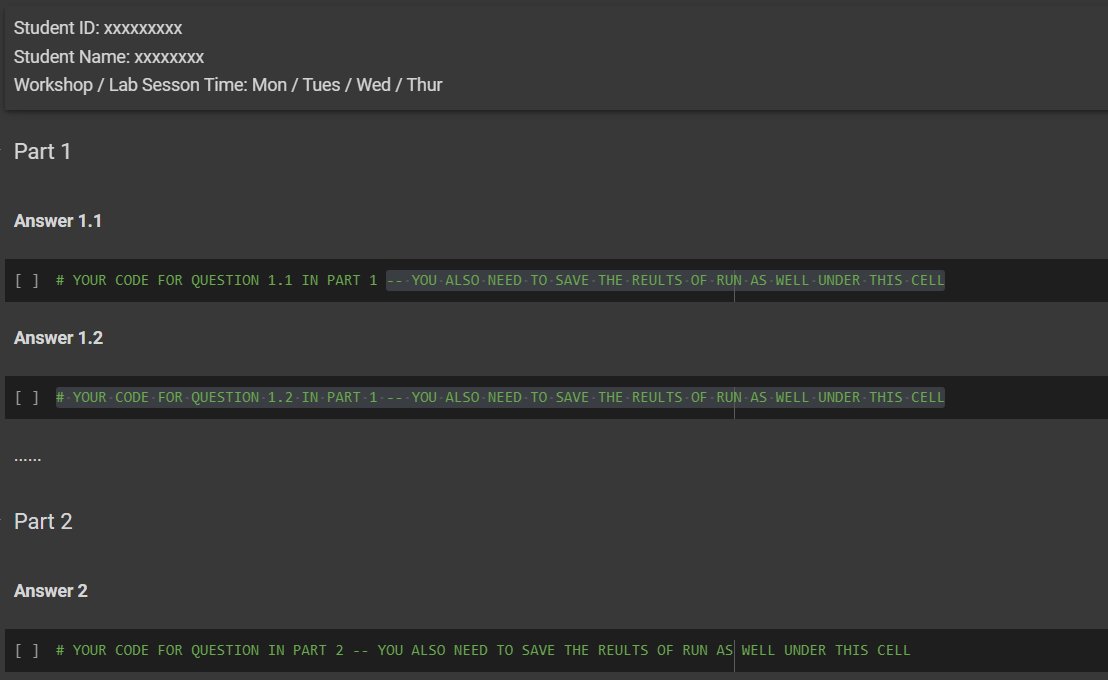
\includegraphics[width=0.8\columnwidth]{figure/assigment1.png}
    \caption{Notebook Format}
    \label{fig:format}
\end{figure}
    

\item[\texttt{SIT742Task1Part2.avi}] (Only if you choose to work on \emph{Part 2} of this assessment task)
A video demonstration between $5$ and $10$ minutes,
and the file format can be other common ones,
such as `\texttt{MKV}', `\texttt{WMV}', `\texttt{MOV}' etc. 

If you are aiming to achieve `\texttt{High Distinction}' (HD) and choose to work on \emph{Part 2} of this assessment task,
one important submission is a \textbf{short video} 
in which \emph{You} orally present the solutions 
that you provide in the notebook 
and illustrate the running of code line by line.

\item[\texttt{SIT742Task1Part2report.pdf}] (Only if you choose to work on \emph{Part 2} of this assessment task)
A short essay report with no more than 500 words,
and the file format can be other common ones,
such as `\texttt{.doc}', `\texttt{docx}' etc.

If you are aiming to achieve `\texttt{High Distinction}' (HD) and choose to work on \emph{Part 2} of this assessment task,
another important submission is a \textbf{short essay} 
in which \emph{You} will explain the code you wrote for the solution,
any of the resource or material which has been helpful 
to resolve the problem, 
and illustrate if there is any alternative way to solve the problem.
In addition, you will also need to follow the common essay writing structure which could be found in \url{https://www.deakin.edu.au/students/study-support/study-resources/academic-skills/essay-writing}

\end{description}

% present how you solve the part 2 questions,
%  and detail the .
%     Part 2 of the assignment has two choices,
%     for students who have the student ID on \textbf{odd} number, 
%     you will need to do the first choice,
%     and for students who have the student ID on \textbf{even} number,
%     you will need to do the second choice.
%     \textcolor{red}{If you did not choose the correct one for part 2, you will lose all the marks for part 2}.
    
% \boxedpoints \pointname{ marks}

    % Use `answer` environment to add solutions
    % \begin{answer}[Question 1.1] for example starts an environment formatted
    % % for Question 1.1 
    % Also,
    % we would like you to make a \textbf{short video} from 5 to 10 mins to describe how you solve the questions on part 2 of the assignment (only if you would like to get \textbf{HD} for this assignment. If you did not submit the video, we will take penalty of your marks of part 2 by 50\%)
    % In the video, 
    % you could run the code you write line by line and detail the solutions you provide in the notebook.
    % Part 2 of the assignment has two choices,
    % for students who have the student ID on \textbf{odd} number, 
    % you will need to do the first choice,
    % and for students who have the student ID on \textbf{even} number,
    % you will need to do the second choice.
    % \textcolor{red}{If you did not choose the correct one for part 2, you will lose all the marks for part 2}.
     
    \part{Python Programming}\label{sec:part1}

    There are \textbf{8} questions in this part for total \textbf{80} marks, and each question is for \textbf{10} marks. 
    
    You are required to use \texttt{Google Colab} to 
    finish all the coding in the \textit{code block cell},
    and \textcolor{red}{provide sufficient coding comments},
    and also \textcolor{red}{save the result of running as well}. 
    
    \begin{answer}[Question 1.1] 
        ages = [5,31,43,48,50,41,7,11,15,39,80,82,32,2,8,6,25,36,27,61,31] and the length of the list is 21
        \begin{itemize}
            \item find the average value of age 
            (don't use \texttt{numpy} and do not import other module or library, do not directly use \texttt{math} module functions except the function \texttt{sum});
            \item find the standard deviation from the age list 
            (don't use \texttt{numpy} and do not import other module or library, do not directly use \texttt{math} module functions except the function \texttt{sum})
        \end{itemize} 
        \textbf{Hints:}
        You could firstly create a function for calculating the mean,
        then create the second function for calculate the sum of square deviations of sequence data, then create the thrid one for standard deviation. Check for the steps on how to calculate the standard deviation from \url{https://www.mathsisfun.com/data/standard-deviation-formulas.html}\\
        \\
        Run your defined \textbf{function(s)} to calculate the average value of age and standard deviation of the age from given list
    \end{answer}
    
    \begin{answer}[Question 1.2]
    Writing the code or function to achieve below requirements:
        \begin{itemize}
            \item You are given the heads of two sorted linked lists list1 = [1,2,4] and list2 = [1,3,4]. Merge the two lists in a one sorted list which is [1,1,2,3,4,4]. (don't use \texttt{numpy} or import other module / library);
            \item You are given the heads of two sorted linked lists list1 = [1,2,4] and list2 = [1,3,4]. Merge the two lists in a one sorted list without duplicated elements which is [1,2,3,4]. (don't use \texttt{numpy} or import other module / library);
        \end{itemize} 
    \end{answer}
    
    \begin{answer}[Question 1.3]
    You are required to design the code (by writing code or function) could achieve the mobile number searching mechanism which could allow you to:
    \begin{itemize}
        \item for Four mobile numbers in a list ['10009091003','10008293312','10007838282', '130001002']
        \item print “Yes” when last digit in mobile number is not 3
        \item print “No” when last digit in mobile number is 3
        \item print “Not Valid” when length of the mobile number is small than 11 digits
    \end{itemize}
    (Optional: You could import re to use the regex function)
    \end{answer}
    
    \begin{answer}[Question 1.4]
    You are required to use \texttt{For statement} to 
    print out below \textbf{*} mark in \textbf{5} lines 
    (must use control flow such as \texttt{For statement}). \\
    
    * \\
    ** \\
    *** \\
    **** \\
    ***** \\
   
    Example only (you could use others like While)
    \begin{lstlisting}[language=Python]
For i in range(5):
    #continue to write your code in below#
    \end{lstlisting}
    Please do not directly print it out, you must finish the question with control flow syntax.
    \end{answer}
    
    \begin{answer}[Question 1.5]
    Given list A = [1,2,3,[4,5,['x1',6,[1,2,3,'sit742']]]], 
    writing a function to print 1,2,3,4,5,x1,6,1,2,3,sit742 (must define a function to run, the input for function is list A, run the function and print the results line by line or in one line)
    \end{answer}
    
    
    \begin{answer}[Question 1.6]
    Write the code or function to achieve: \\
    Sort the dictionary list=$[\{'name':a,'age':55\},\{'name':b,'age':30\},\{'name':c,'age':50\}]$ with the value of age (from smallest to largest, you could use default \texttt{sorted} function).
    \end{answer}
    
    
    \begin{answer}[Question 1.7]
    Define two functions to sum your student ID (all numeric digits in the ID) and then find out if the result is an odd number or even number
    there are two functions for you to implement (you must create the below two functions):
    \begin{itemize}
        \item one is \texttt{sum_digits},
        \item another one is \texttt{check_studentid}.
    \end{itemize}
    your code will have two functions as below:

    \begin{lstlisting}[language=Python]
    def sum_digits(studentid):
        #write your code here

        return sum_digits_result
    def check_studentid(sum_digits_result):

        #write your code here
    \end{lstlisting}
   Run your functions to find out the result and the result must illustrate whether the result from function \texttt{check_studentid} is odd or even number (this is critical to be used for \textbf{Question 2}).
    \end{answer}
    
    
    \begin{answer}[Question 1.8]
    Given an array of integers [1, 2, 6, 8], return indices of the two numbers such that they add up to 10.You may assume that each input would have exactly one solution. \\
    \\
    \textbf{Explanation} \\
    Given nums = [1, 2, 6, 8], target = 10, \\
    Because nums[1] + nums[3] = 2 + 8 = 10, \\
    return [1, 3].

    Your code should have a defined function which could take the array \texttt{nums}= [1, 2, 6, 8] as input and run the function to return a list [1,3] (only [1,3])
    \end{answer}
    
    \part{Python Foundations for Data Science}\label{sec:part2}

    This part is for students who are aiming to 
    achieve `\texttt{High Distinction}' (HD) for this assessment task. The \Cref{sec:part2} has been designed for a particular scenario based data science problems.

    There are \textbf{2} version in this part for \textbf{20} marks:
    \textbf{10} marks for coding, \textbf{5} marks for video presentation \texttt{SIT742Task1Part2.avi} 
    (as in~`\textbf{What to Submit}')
    and \textbf{5} marks for the essay \texttt{SIT742Task1Part2report.pdf} (as in~`\textbf{What to Submit}'). 
    \textcolor{red}{You only need to work on one version in this part
    based on the result in \textbf{Question 1.7} (details in \Cref{sec-which}), and working on the wrong one will result in zero for this question}.  
    
    For your question,
    you are required to use \texttt{Google Colab} 
    to finish all the coding in the \textit{code block cell}, 
    provide sufficient coding comments, 
    and also save the result of running.   
    
    \section{Which question for you?}\label{sec-which}

    In here, 
    if your result in Question 1.7 for the function \texttt{check_studentid} returned as odd, you will need to work on the version 1, if result in Question 1.7 for the function \texttt{check_studentid} returned as even, you need to work on the version 2.
    You will also need to print/save the result of the code running for \textbf{Question 1.7} and you need to have the correct answer for \textbf{Question 1.7} to be able to start the \textbf{Question 2}.

    \begin{itemize}
        \item If your answer in \textbf{Question 1.7} is wrong, Eg: the result should be odd but your result in \textbf{Question 1.7} is even and you choose even -- Zero mark for \textbf{Question 2};
        \item If your answer in \textbf{Question 1.7} is wrong, Eg: the result should be odd but your result in \textbf{Question 1.7} is even and you choose odd -- Zero mark for \textbf{Question 2};
        \item If your code in \textbf{Question 1.7} is not running functionally, Eg: the code in \textbf{Question 1.7} has error -- Zero mark for \textbf{Question 2};
        \item If your answer in \textbf{Question 1.7} is correct, Eg: the result should be odd and your result in \textbf{Question 1.7} is odd but you choose even -- Zero mark for \textbf{Question 2};
        \item If you did not have any code for \textbf{Question 1.7} -- Zero mark for \textbf{Question 2};
        \item Only if your code in \textbf{Question 1.7} is running functionally and returns correct answer, your \textbf{Question 2} will be assessed accordingly.
    \end{itemize}
    
    \section{Question $2$ - Version-I}
    
    \begin{answer}[Question 2 Whether the three numbers could form a triangle?]
    
    Whether the three numbers could form the triangle? You need to write  code (function) with 3 numeric inputs and then check whether the given three numbers could form the triangle. \\
    \\
    \textbf{Question 2.1}
    You are given three sets of list and each list contains three numbers, you will need to write a code with functionality of inputting the three numbers from each list and find out the answers for below (three) questions.
    $list1 = [1,3,5]$, $list2 = [12,35,37]$, $list3 = [2,2,2.8]$
    \begin{itemize}
        \item Define a function to check whether the given three numbers could form the 
        a triangle?
        \item Define a function to check whether the given three numbers could form the right triangle?

        \item Write the code or function to check whether the given three numbers could form the isosceles triangle?

        \begin{description}
            \item[One possible solution] 
            you may try to first define a function to check whether the three input numbers could meet the triangle rule (The sum of the length of the two sides of a triangle is greater than the length of the third side).
            Then you need to check whether the length of the side could meet the condition of right triangle and isosceles right triangle.
        \end{description}     
    \end{itemize}

    Run your code with each list by inputting the numbers and return the results to answer above three questions (you could run your code three times and save the results).
    
    
    \textbf{Question 2.2}
    
    The problem for \textbf{Question 2.2} is how to calculate the area of the triangle. When you find out the list(s) in \textbf{Question 2.1} which could form the triangle, could you also please calculate their area (round to integer)?
    There is one method to calculate the area of given shape 
    - \texttt{Heron's formula} as below:
   \begin{equation} \label{eq:area}
        A = \sqrt{s(s-a)(s-b)(s-c)}
    \end{equation}
    where $s =  \frac{a+b+c}{2}$\\
    
    You are required to define the function \texttt{find_area(a,b,c)} for this problem, 
    and you will need to run the \texttt{find_area()} and print the results for the list(s) in \textbf{Question 2.1}
    which could form the triangle.

    \end{answer}
    
    
    \section{Question $2$ - Version-II}
    
    \begin{answer}[Question 2 The Monty Hall problem -- Do you want to switch the door?]
    
    Suppose you're on a game show, and you're given the choice of three doors: Behind one door is a car; behind the others, goats. You pick a door, say No. 1, and the host, \textbf{who knows what's behind the doors}, opens another door, say No. 3, which has a goat. He then says to you, "Do you want to pick door No. 2?" Is it to your advantage to switch your choice? Scenario is as in \Cref{fig:even}:
    \begin{figure}[H]
        \centering
        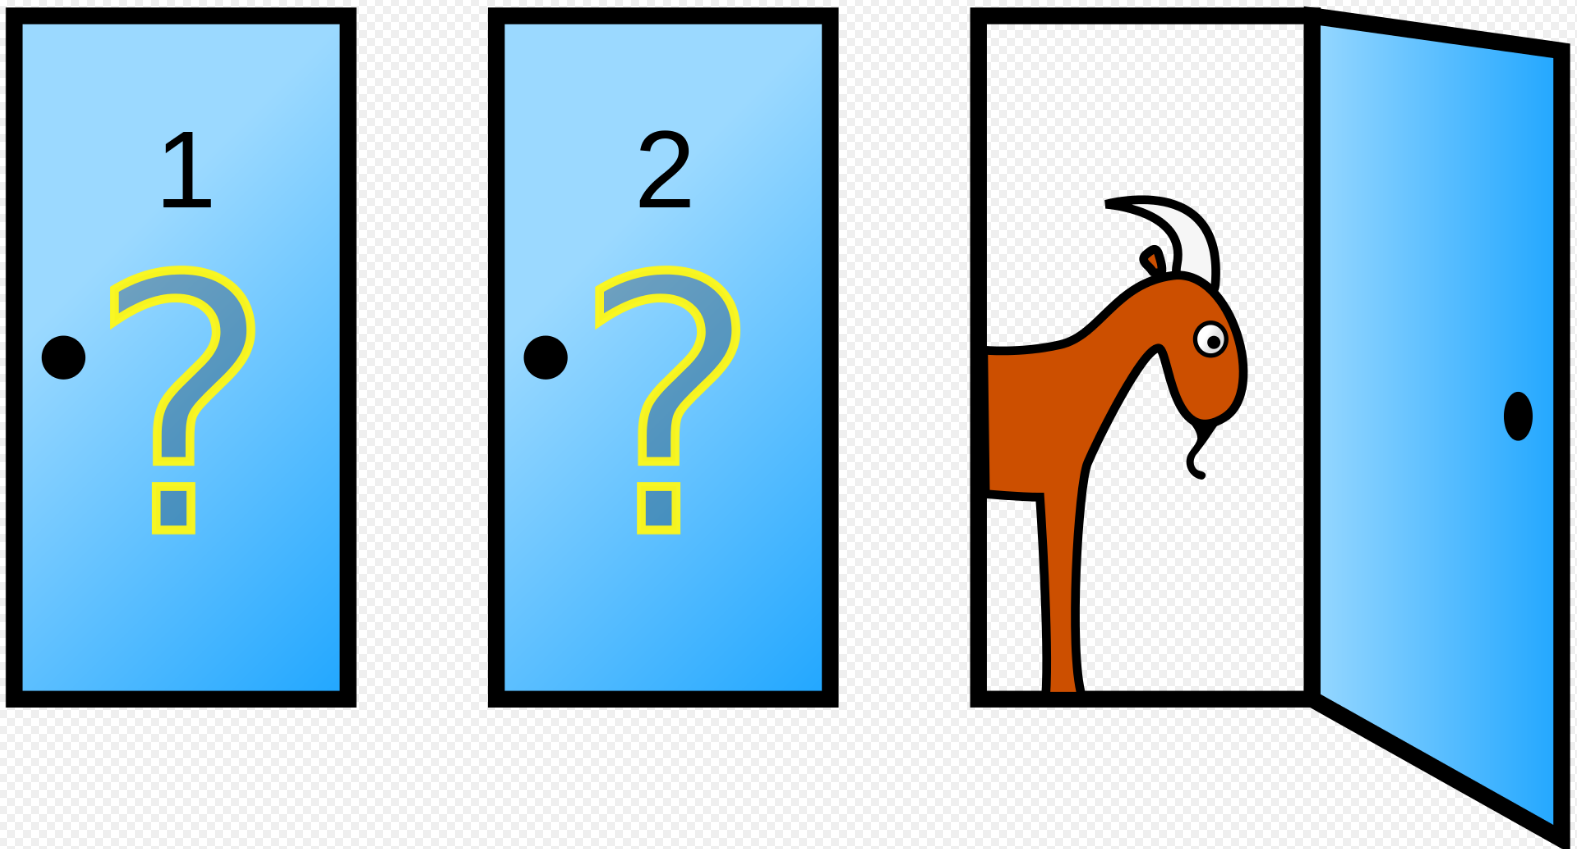
\includegraphics[width=0.65\columnwidth]{figure/monte_hall.png}
        \caption{In search of a new car, the player picks a door, say 1. The game host then opens one of the other doors, say 3, to reveal a goat and offers to let the player switch from door 1 to door 2.}
        \label{fig:even}
    \end{figure}
    

    \textbf{Question 2.1}
 
    You will need to write a code to find out what is the probability to get the car if you switch the door?
    \begin{description}
            \item[One possible solution] 
            You first want to define a variable with random choice to indicate which door has the car.
            Then you need to also define a variable with random choice to indicate the choice that challenger has selected.
            Then host will need to pick the door that is not same as the challenger's choice and also did not has the car.
            Then you need to write the condition to judge whether the other door that challenger did not pick has the car or not. 
            Then repeating the above for $n$ times for calculate the probability.
        \end{description} 
    
           
    \end{answer}
    
    
\end{document}
